\documentclass[a4paper,11pt,titlepage,uplatex]{jsarticle}
\usepackage{report}
\renewcommand{\thesection}{1-\arabic{section}}
\title{Chapter1}
\author{20B01392 松本侑真}
\date{\today}
\begin{document}
\maketitle
\begin{abstract}

\end{abstract}
\tableofcontents
\newpage

\section{General Properties of Nuclei}
\setcounter{section}{3}

\subsection{Nuclear radius and nuclear density}
原子核の大きさは核子数$A$に依存する。原子核半径$R$は
\begin{equation}
	R = r_0A^{1/3},\,r_0 = \SI{1.2}{fm} = \SI{1.2e-15}{m}
	\label{eq:R}
\end{equation}
と表される。
上式から、原子核の体積($4\pi R^3/3$)は$A$に比例し、中心部の密度は核子数$A$にほぼよらず一定値を取ることがわかる。これを密度の飽和性と呼ぶ。
すなわち、核子間には非常に大きな力(\SI{1}{cm^3}あたり1億トン程度)がかかるが、押しつぶされないことがわかる。

実際には、核物質密度として知られる値($\rho_0 \sim \SI{0.16\pm 0.02}{nucleons/fm^3}$:水の密度の\num{3e14}倍)を超えて圧縮させる場合、
ブラックホールや、超新星爆発前の巨大な恒星の重力崩壊のような極限状態に至る必要がある。
この場合、中性子星の典型的な質量と半径($1M_{\odot} \sim \SI{e30}{kg},\,R \sim \SI{10}{km} = \SI{e6}{cm}$)と同じ桁の大きさになる:
\begin{equation}
	\rho = \frac{M_{\odot}}{4\pi R^3/3}\sim \frac{\SI{e30}{kg}}{\SI{4e18}{cm^3}} \sim \rho_0
\end{equation}

有限の核子で構成される原子核では、$\rho_0$よりも密度がやや小さい。式\eqref{eq:R}を用いると、$\rho\sim\SI{0.12}{nucleons/fm^3}$となる。
(\SI{1}{nucleons}とは何を表しているのでしょうか?以下の計算のように、陽子1つの質量が\SI{1}{nucleons}ではなさそうだと思いました。)
\vskip\baselineskip
\begin{tcolorbox}[
		colback = white,
		colframe = green!35!black,
		fonttitle = \bfseries]
	\begin{equation}
		\frac{4}{3}\pi\qty(r_0A^{1/3})^3\rho  = m_{p}A \longrightarrow \rho = \frac{3m_p}{4\pi r_0^3} =0.14m_p \approx \SI{0.12}{nucleons/fm^3}
		\label{eq:0.14}
	\end{equation}
\end{tcolorbox}
このようなことが起きる原因は、拡散表面積(指数関数的に核子密度が0に現象する層)が大きいためである。
一般には、動径方向の依存性を持ったWoods-Saxonモデルと呼ばれる密度分布(Fermi分布)で表現される:
\begin{equation}
	\rho(r) = \frac{\rho_0}{1+\exp{(r-c/z)}}\;。
	\label{eq:woods}
\end{equation}

ここで、$z$は原子核の表面効果による拡散の指標を表すパラメータであり、典型的には$z=\SI{0.5}{fm}$である。
\footnote{たしかに、$\exp(-c/z)\ll 1$が成立しており、$\rho(0)\to\rho_0$となる。}
また、$c$は$\rho(c)=\rho_0/2$で定義される距離である。いくつかの核子における典型的な値は、Table4-1に示されている。

\begin{figure}[H]
	\centering
	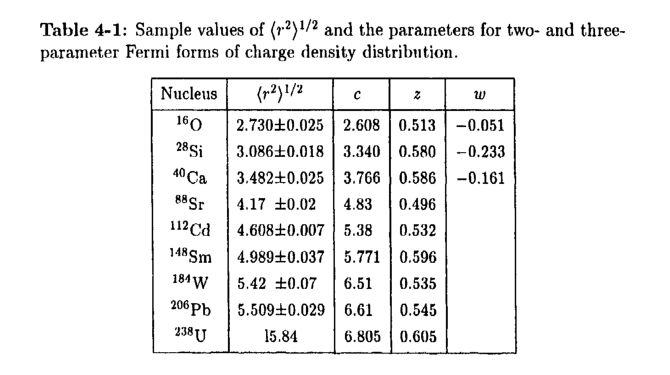
\includegraphics[width=0.6\linewidth]{table4_1.png}
	\caption{核子のパラメータの例(p.112から引用)}
	\label{fig:table4_1}
\end{figure}
なお、平均二乗半径は次のように計算できる:
\begin{equation}
	\ev{r^2} = \frac{3}{4\pi R^3\rho_0}\int r^2\rho(r)dV = \frac{3}{R^3\rho_0}\int_0^\infty r^4\rho(r)dr\quad \qty(= \frac{3}{5}R^2,\,\rho(r)=Const)\;。
\end{equation}

\subsection{Nuclear shape}
安定核は、基本的に球形をしている。4.9章で後で述べるように、これは液滴が表面自由エネルギーを最小化させていることのアナロジーである。
\footnote{水でたとえると、液滴内部の水分子は等方的に周りの水分子からの分子間力を受けて安定するが、表面の水分子は両隣や液滴内部の水分子からしか分子間力を受けない。(気体中の分子密度は液体のそれに比べて低いため。)
	そのため、表面上の分子は液滴内部に引き込まれようとする現象が表面の至る場所で生じている。この結果、表面積を可能な限り小さくしようとする。
	また、体積が一定のとき、表面積が最小になる形状は球なので、分子間力のみがかかっている液滴は球形となる。この証明はどのようにすればいいかわからなかった。(変分法?)}
しかし、たとえば$150<A<190$の原子核の場合、球形からの微小なズレが観測されている。そのズレを表す指標として、
\begin{equation}
	\delta = \frac{\varDelta R}{R}
\end{equation}
というものがある。$R$は式\eqref{eq:R}で与えられる原子核の平均半径であり、
楕円体球形状をしている原子核の場合、$\varDelta R$は長軸方向と短軸方向で異なる値を持つ(球であれば$\varDelta R = 0$)。
原子核では、一般的に$\delta < 0.1$が原子核の低エネルギー状態の場合に成立している。
しかし、2つの原子核を用いた核融合実験では、大きな変形を引き起こすことが可能であり、
$\delta \approx 0.6$程度(長軸半径が短軸半径の2倍)になることが観測されている。
原子核の超変形状態(原子核が非常に高エネルギーのときに生じる状態)の場合については、9.2章で取り上げている。

原子核の変形が引き起こされるひとつの原因として、核子間斥力とクーロン引力の相互作用がある。
クーロン力は距離の二乗に反比例しているため、陽子を可能な限り遠くまで離すことで、原子核は全体のエネルギーを減少させる(結合エネルギーを増やす)ことができる。
体積は一定のままで変形した形状が、結果として好ましくなっている。

一方で核力は、短距離の相互作用がより効果的になるように、原子核を球状に保とうとし、
軽い原子核は核力が強いために全体的に球形をしている。
しかしながら、核子数$A$の値がある閾値を超えると、核子数が増加しても、核力による核子1つあたりの結合エネルギーは増加しなくなる。
その結果、核子の形状がわずかに変形し、クーロン相互作用が減少することで、結合エネルギーを増加させることができる。

\subsection{Density of excited states}
\begin{equation}
	E_B(Z,\,N) = \qty{ZM_{\text{H}} + NM_n -M(Z,\,N)}c^2
	\label{eq:bindingE}
\end{equation}

式\eqref{eq:bindingE}で定義される結合エネルギーは、原子核の基底状態のみで適用される。
一般には、原子核はいくつかの励起状態を取る。
励起状態では、習慣的に基底状態のエネルギーをゼロ点として表される。
異なる原子核のスペクトルを詳しく調べると、核子(nuclei)のスペクトルを調べた場合と似たように、
個々の原子核(nucleus)を特徴づけることができるほど、一意的に決定することが可能である。
個々の特徴に対して、励起状態の分布には、何の価値もない一般的な特徴がある。

原子核は核子によって構成される。
フェルミオンの場合、パウリの排他律によって、それぞれの核子は異なる1粒子状態を占めなければならないことが要請される。
相互作用を無視できる極限では、原子核の基底状態は、核子が最低エネルギー状態から順番に1粒子状態を埋めた状態となる。
これは、全ての分子が全く同じフェルミオンで構成されて、相互作用がない模型であるフェルミ気体模型に類似している。

絶対零度では、フェルミオンは占有可能な1粒子状態のうち最も低いエネルギー状態を占有し、そのうち最もエネルギーが高い状態はフェルミレベルとして知られている。
このような系の励起状態を実現させる唯一の方法は、フェルミ面より下のエネルギー準位を占めているいくつかの粒子を、フェルミ面より上の占有されていないエネルギー準位に押し上げることである。

低エネルギー励起状態では、フェルミ面の少し下に位置するいくつかの粒子を、フェルミ面の少し上の状態に遷移させるエネルギーのみ持っている。
この操作を実行するために利用できる独立した方法はあまり多くないため、状態密度、すなわち単位エネルギーあたりの励起状態の数は少ない。
($E_{\text{F}}$付近の粒子のみが、$E_{\text{F}}$の少し上に励起することしかできないため、取りうる状態数が少ないということですか?)
\begin{figure}[H]
	\centering
	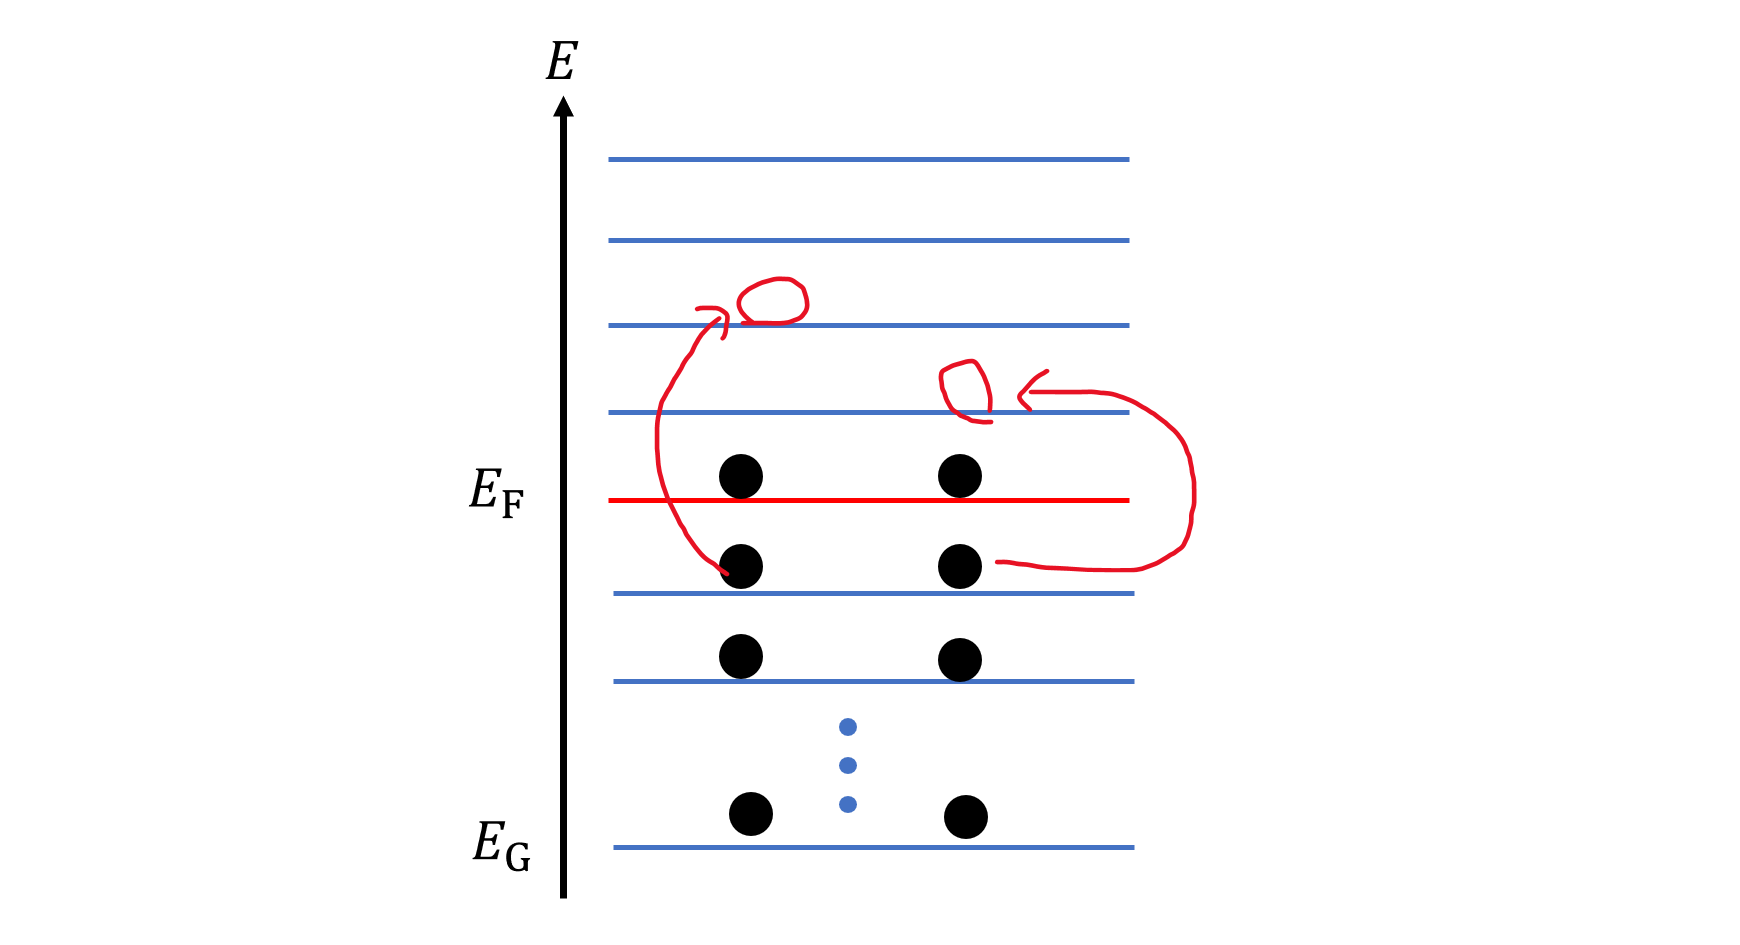
\includegraphics[width=0.5\linewidth]{fermion_state.png}
	\caption{上の文の解釈図}
	\label{fig:fermion_state}
\end{figure}

系の励起エネルギーが上昇していくと、より多くの構成粒子が高エネルギー状態を占有することができ、
多体系の取りうる異なる状態数が上昇していく。その結果、状態密度は増加する。
このような単純な描像に基づいて、Bethe(Hans Albrecht Bethe)は1937年に、励起エネルギー$E$に対応する状態密度の式を導出した:
\begin{equation}
	\rho_{\text{A}}(E) = \frac{1}{12a^{1/4}E^{5/4}}e^{2\sqrt{aE}}\;。
\end{equation}
これは一般にフェルミ気体の式として知られる。$a$の値は密度レベルパラメータである。上式の導出は例えば[152]を参照すれば良い。
\footnote{Google Scholarで書籍は見つけましたが、導出部のページのプレビューが見られなかったです。Betheの原論文も確認しましたが、どこで議論しているのかよくわからなかったです。}
\footnote{講義では、フェルミ気体模型のゾンマーフェルト展開(低温近似)のみを扱ったのですが、上の式は一般の有限温度で成立する式ですか。}
\begin{figure}[H]
	\centering
	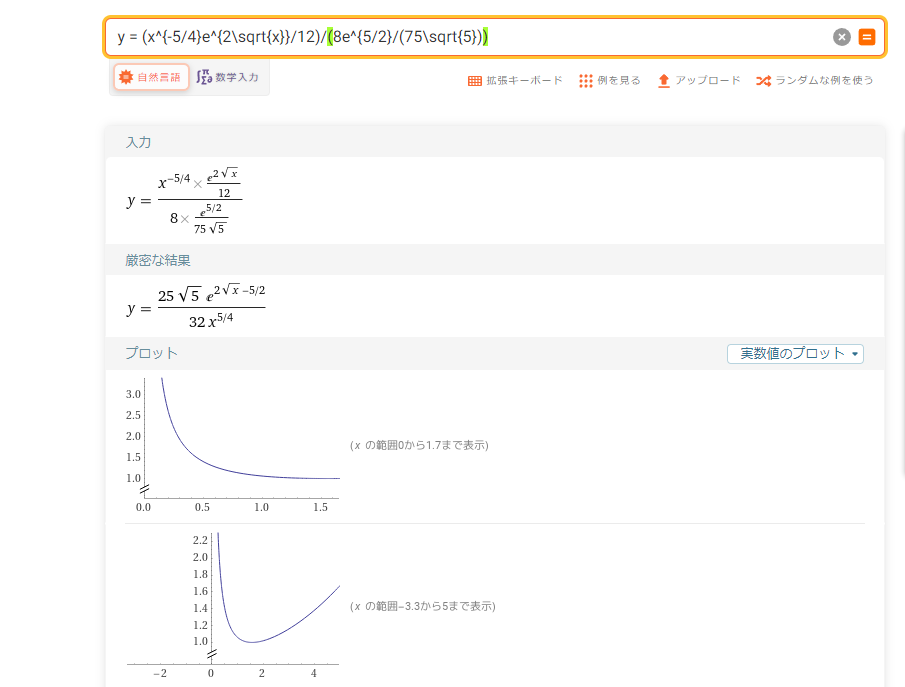
\includegraphics[width=0.65\linewidth]{bethe_E.png}
	\caption{$\rho_{\text{A}}(E)$の概形:励起エネルギーがあまり高くないときには$\rho_A(E)\sim 1$となっている。(極小値が1になるように規格化済み)}
	\label{fig:bethe_E}
\end{figure}

核子間の相互作用によって、単純で滑らかな形状のエネルギースペクトルは修正される。現在では、
各励起状態の位置は、核子間相互作用と核子の複雑な関数となっている。
それにもかかわらず、フェルミ気体模型で与えられた一般形式は、本質的には正しいままである。相互作用の主な影響は、次の二つに分けられる:
\begin{itemize}
	\item 各エネルギー順位の相対的な位置が変化すること
	\item いくつかの$\varDelta$(エネルギーのずれ)によって、全体のエネルギースケールがシフトすること
\end{itemize}

\subsubsection*{一つ目の効果について}
ある特定の観点から見ると、相互作用はフェルミ気体模型に依って与えられる滑らかな形状のスペクトルに対して「揺らぎ」を導入することになる。
興味のある対象によっては、特定のエネルギーレベルもしくはエネルギー準位のグループの位置に注目して研究する場合、揺らぎが重要な要素になる場合がある。
一方で、興味のある対象が、特定の条件下で励起された原子核に蓄積されたエネルギー量などの一般的な特徴である場合、スペクトルの滑らかな部分のみが主な重要性を持つ。

\subsubsection*{二つ目の効果について}
励起エネルギーは基底状態から相対的に計測されるため、後者(基底状態?)に変化があると、全体のスペクトルに一定のシフトが生じる。
一般に、相互作用は非相互作用モデルで与えられる基底状態を下げる傾向にある。このようなエネルギースケールのシフトが生じるために、
状態密度は以下のような式で多く応用される:
\begin{equation}
	\rho_A(E) = \frac{1}{12a^{1/4}(E-\varDelta)^{5/4}}e^{2\sqrt{a(E-\varDelta)}}\;。
\end{equation}
これは、バックシャフトされたフェルミ気体模型の式として知られている。
ここで、$a,\,\varDelta$はそれぞれが調整可能なパラメータとして考えられており、既知のデータに適合するようにフィッティングされる。

\newpage
\subsection{Scattering cross section}
原子核を研究する際には、しばしば1つの粒子を他の粒子に散乱させる手法を用いる。これは、フェムトメートルオーダーの物体を調べる必要があるためである。
可視光の波長は一方でそれよりとても長く、\SI{e-7}{m}程度である。
長さのスケールを短くして素粒子物理学に興味を持つ場合、可視光よりもはるかに短い波長、つまりはるかに高いエネルギーが必要になる。
そしてこれは散乱によって最も容易に実現できる。
所望の長さのスケールに到達するために散乱実験で必要とされるエネルギーの概算値は、対応するドブロイ波長を調べることで得られる
\footnote{Table 1-4の意味がよくわかりませんでした。電子や陽子の運動量によって異なる波長のドブロイ波になり、それに対応する光子の波長があげられていますが、粒子の散乱実験と何が関係あるのでしょうか。}:
\begin{equation}
	\lambda = \frac{h}{p}\xrightarrow[v\to c]{}\frac{hc}{E}\;。\quad\qty(\because E=\sqrt{(mc^2)^2 + (pc)^2}\xrightarrow[v\to c]{} pc \;。)
\end{equation}

\begin{figure}[H]
	\centering
	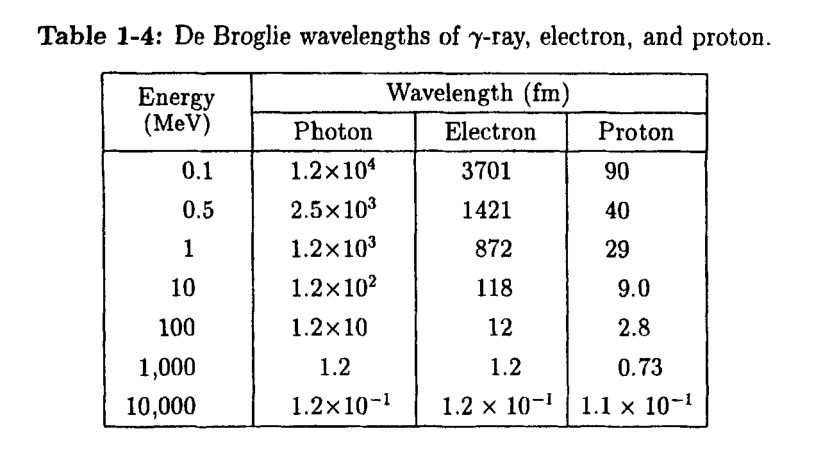
\includegraphics[width=0.8\linewidth]{debroglie.png}
	\caption{各粒子のドブロイ波長}
	\label{fig:debroglie}
\end{figure}

標的粒子によって入射粒子が散乱される確率は、散乱断面積という用語で説明されることが一般的である。全断面積$\sigma$は以下のように定義される:

相互作用の範囲外から標的に向かって直線的に進む粒子を考える。その速度を$v$とすると、粒子は経過時間$t$の間に体積$vt\mathcal{A}$の円柱の軌跡を描く。
なお、$\mathcal{A}$は粒子によって覆われる面積(粒子の断面積)である。散乱確率$P$は、標的粒子によってブロックされる面積と、$\mathcal{A}$によって与えられる。
単位体積あたりの標的粒子数を$n$として、標的粒子の厚さを$T$とする。
\footnote{今は、原子核の核子どれか一つと衝突することを考えているからこのような表現になっているのですか?}
このとき、ビーム粒子(入射粒子)からは$n\mathcal{A}T$の粒子数があるように見える。
よって、散乱確率は
\begin{equation}
	P = \frac{n\mathcal{A}T\sigma}{\mathcal{A}} = \sigma nT
\end{equation}
となる。$n,\,T$は与えられており、次元はそれぞれ長さの3乗の逆数と長さを持ち、$P$は無次元量であるため、全断面積$\sigma$は長さの二乗の次元を持つ必要がある。

全ての散乱粒子を検出する必要があるため、全断面積は実験で直接的に計測されるわけではない。散乱粒子の角度分布は、より多くの情報を提供してくれるため、実際にはより有益な量である。
上記と同じ手法を用いて、微分散乱断面積$\dv*{\sigma}{\Omega}$を、散乱粒子が検出器に入射してきたときの角度$(\theta,\,\phi)$を用いた確率$P(\theta,\,\phi)$と、
標的粒子の中心からの微小な立体角$\varDelta\Omega$を用いて、
\begin{equation}
	P(\theta,\,\phi) = \dv{\sigma}{\Omega}nT
\end{equation}
と定義できる。(つまり、立体角${\Omega}(\theta,\,\phi)$の方向に散乱される確率を用いて、${\Omega}$方向の断面積を$\dv*{\sigma}{\Omega}_{(\theta,\,\phi)}$と表している。)
全断面積と微分断面積は全立体角で積分した以下の式で関係付けられる:
\begin{equation}
	\sigma=\int_0^{4\pi} \dv{\sigma}{\Omega}\dd{\Omega} = \int_0^{\pi}\int_{0}^{2\pi}\dv{\sigma}{\Omega}\sin\theta\dd{\theta}\dd{\phi}\;。
\end{equation}
\S-B2で、反応後の波動関数を用いた微分散乱断面積の再定義を行っている。

\begin{figure}[H]
	\centering
	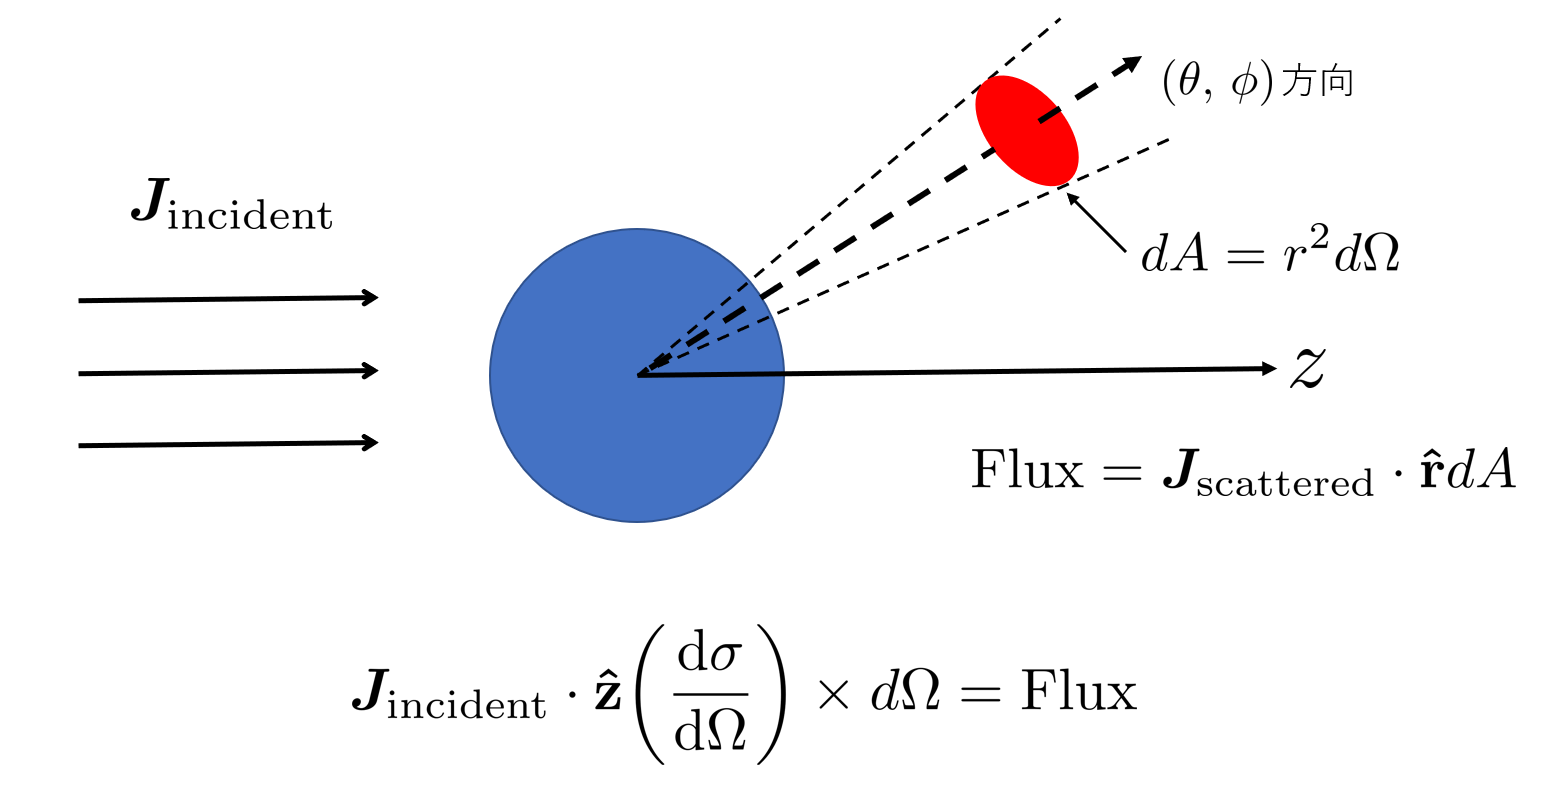
\includegraphics[width=0.8\linewidth]{bibun_sanran_danmenseki.png}
	\caption{微分散乱断面積の図解}
	\label{fig:bibun_sanran_danmenseki}
\end{figure}
微分散乱断面積の意味は上の図のように理解できる。
古典的には、物体との衝突後に立体角$\Omega(\theta,\,\phi)$方向に散乱される入射粒子方向への物体の断面積が$\dv*{\sigma}{\Omega}$である。
それをあらゆる角度について積分したものが全断面積であり、「そこに衝突すれば、どこかの方向へ入射粒子が散乱していく物体の断面積」と解釈できる。
半径$a$の剛体による散乱の全断面積が古典的に$\pi a^2$となるのは、太陽の光が剛体に当たって作る影の大きさに他ならない。
\newpage
\subsection{補足:量子論的な微分散乱断面積の定義について}
\S-B2を確認したところ、量子論的な定義は量子力学3で行ったものと同じであった。つまり、入射粒子の波動関数を
\begin{equation}
	\psi_{\text{incident}}(\bm{r}) = e^{ikz}
\end{equation}
とし、散乱波の$r\to\infty$での漸近形を
\begin{equation}
	\psi_{\text{scattered}}(\bm{r}) = f(\theta,\,\phi)\frac{e^{ikr}}{r}
\end{equation}
とする。($1/r$依存性はShcr\"{o}dinger方程式の解から要請されるもの。)
粒子流は
\begin{equation}
	\bm{J} = -i\frac{\hbar}{2m}\qty(\psi^*\grad\psi - (\grad\psi^*)\psi)
\end{equation}
であり、$\div\bm{J} = \dv*{(\psi^*\psi)}{t} = 0$を満たしている。実際に波動関数を代入すると、
\begin{equation}
	\bm{J}_{\text{incident}} = \frac{\hbar k}{m}\vu*{z},\,\bm{J}_{\text{scattered}} = \frac{\hbar k}{m}\frac{1}{r^2}\abs{f(\theta)}^2\vu*{r} + \order{\frac{1}{r^3}}
\end{equation}
となる。散乱波の微小面積$\dd{A} = r^2\dd{\Omega}$を通過するフラックスは
\begin{equation}
	\bm{J}_{\text{scattered}}\cdot\vu*{r}\dd{A} = \frac{\hbar k}{m}\abs{f(\theta)}^2\dd{\Omega}
\end{equation}
となる。微分散乱断面積は立体角あたりの散乱フラックスと入射フラックスの比であるから、散乱振幅が求まればその値($=\abs{f(\theta)}^2$)が求まることになる。
散乱振幅は、波動関数の部分波展開$\psi(r,\,\theta) = \sum_{l=0}R_l(r)P_l(\cos\theta)$が可能であることから求まる。
なお、$P_l(\cos\theta)$はLegendre多項式であり、$l$は角運動量の量子数である。計算を進めると、
\begin{equation}
	\psi_{\text{incident}} = \sum_{l=0}^{\infty}\frac{2l+1}{2ik}\qty[\frac{e^{ikr}}{r}-(-1)^{l}\frac{e^{-ikr}}{r}]P_l(\cos\theta)
\end{equation}
となる(Rayleighの公式)。
散乱理論によると、散乱振幅は波動関数が
\begin{equation}
	\psi(\bm{r}) = e^{ikz} + f(\theta)\frac{e^{ikr}}{r},\,r\to\infty
\end{equation}
によって定義された。散乱振幅を(係数がきれいにまとまるように)
\begin{equation}
	f(\theta)=\sum_{l=0}^{\infty}\frac{2l+1}{k}f_lP_l(\cos\theta)
\end{equation}
と部分波展開すると、波動関数の漸近形は以下のようになる:
\begin{equation}
	\psi(\bm{r})\sim \sum_{l=0}^{\infty}\frac{2l+1}{2ik}
	\qty[(-1)^{l+1}\underset{内向き球面波}{\underline{\frac{e^{-ikr}}{r}}}
		+\underset{S行列:S_l}{\underline{(1+2if_l)}}\frac{e^{ikr}}{r}]P_l(\cos\theta)\;。
\end{equation}
S行列のユニタリ性より、位相のずれ$\delta_l$を用いて
\begin{equation}
	S_lS_l^{\dagger} = 1 \Leftrightarrow S_l = e^{2i\delta_l}
\end{equation}
と書ける。これより、部分波展開の係数が求まる:
\begin{equation}
	f_l = e^{i\delta_l}\sin\delta_l\;。
\end{equation}
この式より、
\begin{equation}
	f(\theta) = \frac{1}{2ik}\sum_{l=0}^{\infty}(2l+1)e^{i\delta_l}\sin\delta_lP_l(\cos\theta)
\end{equation}
を得る。Legendre多項式の直交性を用いると、全断面積$\sigma_{\text{T}}$は
\begin{equation}
	\sigma_{\text{T}} = 2\pi\int_{-1}^{1}\dd{(\cos\theta)}\dv{\sigma}{\Omega} = \frac{4\pi}{k^2}\sum_{l}(2l+1)\abs{f_l}^2 = \frac{4\pi}{k^2}\sum_{l}(2l+1)\sin^2\delta_l
\end{equation}
となる。特に、標的が半径$a$の剛体球ポテンシャルの場合、($r\geq a$では$V=0$より)動径方向のSchr\"{o}dinger方程式の解が球Bessel関数で与えられることから、長波長極限を取ると$\sigma_T = 4\pi a^2$となる。これは、波動関数の回折が生じていることを表している。
(古典的に考えれば$\sigma_T=\pi a^2$になるはず。)

\subsection{Reaction types}
我々が扱いたい反応のうち、最終的な状態は通常二体間の反応である。言い換えれば、反応前は発射粒子$a$が標的粒子$A$に入射される。
反応後は、粒子$b$が散乱され、粒子$B$が残される。この反応は次の2つの方法のうちどちらかで表現される:
\begin{equation}
	A(a,\,b)B\qquad \text{or} \qquad a+A\longrightarrow b+B\;。
\end{equation}
たとえば、陽子を発射して\ce{^{48}Ce}をターゲットとする。そして中性子が反応によって出現されることが観測され、\ce{^{48}Sc}が残る。
この反応は
\begin{equation}
	\ce{^{48}Ca}(p,\,n)\ce{^{48}Sc}\qquad\text{or}\qquad p+\ce{^{48}Ca}\longrightarrow n+\ce{^{48}Ce}
\end{equation}
と表現される。標的粒子である\ce{^{48}Ca}が陽子ビームに照射される際に、他の反応が起こる可能性がある。
例えば、陽子が出現し、\ce{^{48}Ce}が励起状態になる場合である。この反応は
\begin{equation}
	\ce{^{48}Ca}(p,\,p')\ce{^{48}Ce^*} \qquad\text{or}\qquad p+\ce{^{48}Ca}\longrightarrow p'+\ce{^{48}Ca^*}
\end{equation}
と表される。ここで、アスタリスクは反応後を表し、\ce{^{48}Ca}は励起状態に遷移している。
プライムがついている陽子は、そのエネルギーが入射してきた陽子のそれとは異なることを表している。

これらの組み合わせは、それぞれ陽子-\ce{^{48}Ca}散乱の異なる出口チャンネル(exit channelの訳がわかりませんでした。)であり、可能な、つまり「開いた」出口チャンネルは、
散乱時の保存則と選択則によって支配されている。一般に、反応において可能となる開いたチャンネル数は、エネルギーが上昇すると急激に増加する。

許された出口チャンネルは、2つの粒子からなる最終状態によって制限されるものではない。たとえば、上の例では陽子の代わりに重陽子が用いられることがある。
出口チャンネルとして考えられるのは、重陽子が陽子と中性子に分解されるものもある。このような反応は
\begin{equation}
	\ce{^{48}Ca}(d,\,pn)\ce{^{48}Ca}\qquad\text{or}\qquad d+\ce{^{48}Ca}\longrightarrow p+n+\ce{^{48}Ca}
\end{equation}
と表される。議論を簡単にするために、最終的に3つ以上の粒子を含む反応はほとんど無視することにする。
さらに、発射核と標的核、散乱粒子と残留核の区別は、標的が実験室内で静止している固定標的実験にのみ有効である。
入射チャンネル内の2つの粒子が互いに向かって移動する衝突ビーム実験では、この分離は意味を持たない。
ほとんどの議論では、2体系の質量中心でのものであり、その際の区別は単なる意味合いの問題に帰結される。

弾性散乱では、入射粒子と標的粒子の両方がもともとの状態に留まったままである。通常は、それぞれの基底状態である。
弾性散乱は、一般的には反応の観点から最もシンプルなものである。
たとえば、電子の弾性散乱は原子核の電荷密度分布のマッピングに用いられる。
相互作用は主に電磁気的なものであるため、核の電荷分布が点電荷とどのように異なるかを結果から推察することができる。

非弾性散乱とは、入射した運動エネルギーの一部が、反応に巻き込まれた原子核の励起や新たな粒子の生成に使われる散乱である。
最もわかりやすい例は、電磁気的な相互作用によって標的原子核を励起状態にするクーロン散乱であり、これは電磁気的な崩壊の逆反応である。
他の例として、
\begin{equation}
	\nu_e + \ce{^{37}Cl}\longrightarrow e^- + \ce{^{37}Al}
\end{equation}
の反応は、\ce{^{37}Ar}のベータ崩壊の逆反応であり、太陽ニュートリノの検出に用いられている。

2つの原子核が相互作用するとき、1つ以上の核子を互いの原子核に移動させることが可能である。
例えば、重陽子を入射させ、標的粒子を\ce{^{16}O}とすると、重陽子中の緩く結合した中性子が標的の原子核に引き寄せれられ、付着してしまうことがある。
散乱後の粒子は陽子となり、残留する原子核は\ce{^{17}O}となる。
このような反応($\ce{^{16}O}(d,\,p)\ce{^{17}O}$)は、剥離反応(stripping reaction)と呼ばれ、
中性子が入射粒子から剥離されている。逆反応はピックアップ反応(pickup reaction)であり、例えば\ce{^{17}O}(\ce{^{3}He},\,\ce{^{4}He})\ce{^{16}O}がある。
ここで、標的粒子\ce{^{17}O}内部の中性子は入射粒子\ce{^{3}He}に拾われる。散乱粒子は\ce{^{4}He}となり、残留粒子は\ce{^{16}O}である。
より複雑な核子移動も重イオン元素を用いれば誘起される場合がある。

核融合は、核子移動反応の極端なものであると考えることができる。
この場合、2つの重イオンを近づけることで、2つのイオンの核子間に核力が働き、中間状態である複合原子核が形成される。
好条件下では、ガンマ線や核子を放出することで、系内の余剰エネルギーを捨てることができ、核(基底状態の原子核という意味?)とみなせる最終状態が得られるかもしれない。
例えば、まだ名づけられていない超重元素\ce{^{277}112}(コペルニシウム:Cn)は、\ce{^{208}_{82}Pb}を標的粒子として、\ce{^{70}_{30}Zn}を入射させて得られた。

あるいは、最終状態が既知の原子核の中で異常な状態である場合もある。
2つの重イオンの衝突が多くの角運動量を伴うため、最終状態はかなりの割合で保持され、高スピン状態になる可能性が高い。
例えば、\ce{^{155}_{64}Gd}(\ce{^{16}_{8}O},\,\ce{4n})\ce{^{167}_{72}Hf}の反応は、\ce{^{16}O}と\ce{^{155}Gd}が融合することで\ce{^{167}Hf}原子核が生じる。
4つの中性子といくつかのガンマ線が持っていく角運動量を無視すると、最終状態の系において取りうる値を推測できる。
\ce{^{16}O}ビームの重心系エネルギーを$E_{\text{cm}}=\SI{75}{MeV}$として、衝突径数を$b=\SI{10}{fm}$とする。
その結果、古典的な定義式$\bm{l}=\bm{r}\cross\bm{p},\,\bm{p}=m\bm{v}$を元にして、
\begin{equation}
	l=mv_{\text{cm}}b = b\sqrt{2mE_{\text{cm}}}\sim 80\hbar
\end{equation}
を得る。(系の初期状態の角運動量)
\vskip\baselineskip
\begin{tcolorbox}[
		colback = white,
		colframe = green!35!black,
		fonttitle = \bfseries]
	\begin{align}
		l & \sim \frac{b}{c}\sqrt{2\times16(m_{p}c^2)E_{\text{cm}}} = \frac{\SI{10e-15}{m}}{\SI{3e8}{m/s}}\sqrt{2*16(\SI{511}{keV}*1800)\SI{75}{MeV}} \notag        \\
		  & = \frac{4}{3}\times\SI{e-22}{s}\sqrt{2^2*9*500*10^{-3}*75}\,\si{MeV} = 40\sqrt{150}\times 10^{-22}\si{MeV.s} = 480\times10^{6}*\SI{1.6e-41}{J.s} \notag \\
		  & = \SI{76.8e-34}{J.s}\sim 80\hbar\quad\because \hbar\sim \SI{1e-34}{J.s}
	\end{align}
\end{tcolorbox}

これは、この方法で生じる\ce{^{167}Hf}で観測されている、$(73/2)\hbar$のような高スピン状態を実現するために十分な値である。
これと比べて、\ce{^{167}Hf}の基底状態におけるスピンはたった$(5/2)\hbar$である。
たった167個の核子で構成されている原子核で、このような巨大なスピンが存在することができる唯一の方法は、核子のかなりの割合が一貫して独立的に振舞うことである。(核子のスピン$\hbar/2\times 167$ということ?)
これは、通常は基底状態で観測される、球形に近い核形状からかけ離れた核の集団行動の例である。

このようなエキゾチック状態を作り出すためには、2つのイオン間のクーロン障壁を克服するのに十分なエネルギーが必要であることが一般的である。
これは、核融合が起こるために、2つの核子集団が衝突するために必要なことである。
同時に、寿命を長くして最終状態を検出したいために、余剰分を捨てなければいけないため、系に必要以上のエネルギーを注入したくない。
$E_{\text{cm}} = \SI{75}{MeV}$の値は、\ce{^{16}O}のような軽いイオンに対して実際に使用されている値とほぼ同じである。
$b=\SI{10}{fm}$の値もまた、合理的な選択である。なぜなら、イオンが接触しているときの、2体の中心間の距離の半分を表しているからである。
\footnote{酸素原子核の大きさが\SI{10}{fm}程度だとわかりましたが、今回は標的が重イオンなので、$b=\SI{10}{fm}$とするのが合理的なのかがわかりませんでした。$b\leq r_a+r_b$が成立すればいいという認識です。}

\section{Commonly Used Units and Constants}
原子核では、日常生活における通常のスケールと比べて長さが非常に短く、時間が非常に短いスケールを扱っている。
メートルよりも適している長さの単位は、既にみているように、\si{fm}と略記されるフェムトメートル(\SI{1}{m} = \SI{e-15}{fm})がある。
たとえば、原子核の典型的な長さは\SI{1}{fm}のオーダーである。同時に、核力の実効的な長さでもある。
核反応の反応断面積は、\SI{e-28}{m^2}と等しい組立単位であるbarnがよく用いられる。
典型的な値はミリバーンであり、$\SI{1}{mb} = \SI{e-3}{b} = \SI{e-1}{fm^2}$である。

原子核物理には、さまざまな時間スケールが入り込む。Table 1-1でみたように、強い相互作用の典型的な反応時間は\SI{e-23}{s}である。
それと対極的なスケールは、太陽系が形成される前に作られた天然の放射性元素で見つけられる。
これらの放射性核種の寿命は、$10^9$年以上のオーダーであることが必要である。なぜなら、寿命がより短いものはほとんど崩壊してしまっているからである。

\SI{e-15}{s}から\SI{e-23}{s}までのスケールの寿命を持つ状態に対しては、エネルギー分布の幅である$\Gamma$が寿命の特徴として使われることがある。
不確定性原理によると、$\varDelta E\varDelta t = \hbar$となる。$\varDelta t$の時間にだけ存在する状態は、$\varDelta E \sim \hbar/\varDelta t$
以下の不確かさまでしかそのエネルギーを測定することができない。
これは、観測された状態のエネルギーの確率分布に幅$\Gamma = \hbar/\overline{T}$を持たせている。
ここで、$\overline{T}$は状態の寿命(平均寿命)である。$\hbar=\SI{6.58e22}{MeV.s}$であるため、$\Gamma\sim \SI{100}{MeV}$のとき、寿命のオーダーは\SI{e-23}{s}
であり、$\Gamma\sim\SI{1}{eV}$のとき、寿命のオーダーは\SI{e-15}{s}である。

核子の質量は\SI{1.67e-27}{kg}であり、中性子は陽子より\SI{0.14}{\percent}だけ重い。質量の便利な単位は原子質量単位であり、\si{u}や\si{amu}と略され、$\SI{1}{u}=\SI{1.6605402e-27}{kg}$である。
これは、中性の\ce{^{12}C}原子を標準として定義される
\footnote{\si{mol}の定義が2019年から変わったため、この値は不正確。
	さらに、2019年の国際単位系国際文書にて、原子質量単位はSI併用単位ではなくなったため、現在では代わりに\si{Da}(ダルトン)が用いられる。\si{u}は、\si{Da}と同じ単位の別称(と記号)と注記されているのみである。}:
\sisetup{separate-uncertainty=false}
\begin{equation}
	\si{u} = \frac{\text{\ce{^{12}C}原子の質量}}{12} = \frac{\SI{1}{kg}}{N_{\text{A}}} = \SI{1.6605402(10)e-27}{kg} = \SI{931.49432(28)}{MeV/c^2}\;。
\end{equation}
ここで、$N_{\text{A}} = \SI{6.60221367(37)e26}{(kg.mol)^{-1}}$はアボガドロ数であり、カッコ内の数値は下一桁の不確実性を表している
\footnote{2019年までは、炭素12が\SI{12}{g}のときの物質量が\SI{1}{mol}と定義されており、そのためアボガドロ数に不確実性があった。
	2019年以降はアボガドロ定数を正確に\SI{6.02214076e23}{/mol}と定義したため、\SI{1}{mol}の炭素12の質量は\SI{12}{g}ではなくなった。}。
これを用いると、自由な陽子と中性子の質量は
\begin{equation}
	M_p = \SI{1.007276470(12)}{u},\qquad M_n = \SI{1.008664898(12)}{u}
\end{equation}
である。この定義では、\ce{^{12}C}の質量は厳密に\SI{12}{u}である。

結合エネルギーは原子核の静止質量エネルギーのごく一部なので、原子質量単位での値は、核子の数$A=N+Z$と数値的にほとんど変わらない。
核の質量を質量超過(質量欠損とも呼ばれる)$\varDelta(Z,\,N)$で表すと便利なことがあり、以下のルールで定義される:
\begin{equation}
	\varDelta(Z,\,N) \coloneqq \qty{M(Z,\,N) - A}\times\SI{931.49432}{MeV}\;。
\end{equation}
ここで、$M(Z,\,N)$は$Z$個の陽子と$N$個の中性子からなる原子核の質量(単位は\si{u})である。
定数$931.49432$は、原子質量単位から\si{MeV}への変換定数である。水素原子であれば、質量超過は
\begin{equation}
	\varDelta(\ce{H}) = \qty(1.007276470-1)\times 931.49432 + 0.51110 = \SI{7.2891}{MeV}
\end{equation}
である。(なぜここでは上の定義式通り、$M(1,\,0)-A$で計算せず、陽子単体の質量と電子の質量を別に足しているのか。
ここでは陽子と電子の結合エネルギー(第一イオン化エネルギー)$\SI{13.6}{eV}$を無視している?)
自由な中性子では
\begin{equation}
	\varDelta(\ce{n}) = \qty(1.008664904-1)\times 931.49432 = \SI{8.0713}{MeV}
\end{equation}
である。(なぜ$M(0,\,1)$が$M_n$と一致していないのか??)
質量超過を用いると、結合エネルギーは
\begin{equation}
	E_{B}(Z,\,N) = Z\varDelta(\ce{H}) + N\varDelta(n) - \varDelta(Z,\,N)
\end{equation}
と表記できる。
\vskip\baselineskip
\begin{tcolorbox}[
		colback = white,
		colframe = green!35!black,
		fonttitle = \bfseries]
	$M$は\si{MeV/c^2}単位の質量で、$m$を\si{u}単位の質量とする。\SI{1}{u} = \SI{931.49432}{MeV}なので、
	\begin{align}
		E_{B}(Z,\,N) & = \qty{ZM_\text{H} + NM_n - M(Z,\,N)}c^2 = \qty{Zm_{\text{H}} + Nm_{n} - m(Z,\,N)}\times{\SI{931.49432}{MeV}} \notag \\
		             & = \qty{(Zm_{\text{H}} - Z) + (Nm_n-N) -\qty(m(Z,\,N) - A)}\times{\SI{931.49432}{MeV}} \notag                         \\
		             & = Z\varDelta(\ce{H}) + N\varDelta(n) - \varDelta(Z,\,N)
	\end{align}
	となる。
\end{tcolorbox}
いくつかの結合エネルギー表の中には、その値が質量超過の項によって与えられている。

質量の代わりに、それと等しい静止質量エネルギーを用いて作業する方が好ましい場合もある。
既にみたように、原子核物理学では、通常\si{MeV}や\si{eV}(\SI{1}{MeV} = \SI{1.60217733e-13}{J})の単位を使う。
例えば、中性子の質量エネルギーは\SI{939.56563}{MeV}である。
いくつかの高エネルギー現象にとっては、\si{MeV}の1000倍大きい単位である、\si{GeV}(\SI{e9}{eV})を代わりに用いる方がより適している。
例えば、核子の質量エネルギーのオーダーは\SI{1}{GeV}である。
磁気双極子モーメントを表す核磁子の大きさ$\mu_N$のように、核子の他の特性を測る組立単位もいくつか使われている。
議論に登場するそれぞれの値を定義しよう。
プランク定数$h$や光速$c$、素電荷$e$などの普遍的な物理定数は、原子核に関する計算に非常によく出てくる。
電荷量については、陽子のもつ電荷量である$e$を単位とする。
プランク定数については、ほとんどの状況において$\hbar=h/2\pi$を使う方がより便利だとわかっている。
実際に、$\hbar c = \SI{197.3}{MeV.fm}$の組み合わせは、いろいろな計算に自然に入ってくる。
例えば、ドブロイ波長に関する以前の議論では、次のように$\hbar c$の項を用いると、より簡単に計算ができる:
\begin{equation}
	\lambda = \frac{h}{p} = \frac{2\pi \hbar c}{pc}\xrightarrow[v\to c]{} \frac{2\pi\hbar c}{E}\;。
\end{equation}
ここで、$p$は粒子の運動量、$E$は粒子のエネルギーである。
同様にして、衝突計数$b$における2つの重イオン衝突による角運動量$l$の値の推定では、$\hbar$を単位とした値の評価は
\begin{equation}
	\frac{l}{\hbar} = \frac{mv_0b}{\hbar} = b\frac{\sqrt{2mE}}{\hbar} = b\frac{\sqrt{2mc^2E}}{\hbar c}
\end{equation}
とできる。最終的な式で見られるように、質量は静止質量エネルギー$mc^2$に変換されて、分母は$\hbar c$になっている。
\vskip\baselineskip
\begin{tcolorbox}[
		colback = white,
		colframe = green!35!black,
		fonttitle = \bfseries]
	適当に計算しやすい値に丸めて概算すると以下のようになる:
	\begin{equation}
		mc^2 = 16*\SI{938}{MeV},\,E = \SI{75}{MeV},\,b=\SI{10}{fm}\longrightarrow
		\frac{l}{\hbar} \approx 10*\frac{\sqrt{2*16*900*75}}{200}
		= 30\sqrt{6} = 75\;。
	\end{equation}
\end{tcolorbox}

電磁気学に関する方程式はcgs単位系とSI単位系の混在により、複雑になっている。
式をcgs単位系からSI単位系に「変換」するための「余分な」因子を角括弧に入れて書くことにする。
つまり、因子が含まれていない場合はcgs単位系で、含まれている場合はSI単位系で式が成立している。
したがって、片方の電荷が$ze$、もう片方の電荷が$Ze$であり、距離が$R$だけ離れた2粒子間の静電ポテンシャル$V_C(R)$は、
\begin{equation}
	V_C(R) = \qty[\frac{1}{4\pi\varepsilon_0}]\frac{(ze)(Ze)}{R}
\end{equation}
で与えられる。
各括弧内の因子を無視すればcgs単位系で、因子を無視しなければSI単位系で式が成立している。
電磁気学が採用する単位系による依存性を避けるために、微細構造定数
\begin{equation}
	\alpha = \qty[\frac{1}{4\pi\varepsilon_0}]\frac{e^2}{\hbar c} \approx \frac{1}{137}
\end{equation}
を用いて、式を書き換えることができる。したがって、
\begin{equation}
	V_C(R) = \frac{\alpha\hbar c}{e^2}\frac{(ze)(Ze)}{R} = \alpha\hbar c\frac{zZ}{R}\approx 1.44\frac{zZ}{R(\si{fm})}\,\si{MeV}
\end{equation}
となる。$\alpha\hbar c \approx\SI{1.44}{MeV.fm}$とsたため、最右辺の$R$はフェムトメートルの単位で与えられる。
似たような手法で、$Z$個の陽子を持つ半径$R$の球状原子核の静電ポテンシャル(Coulomb energyとありますが、静電ポテンシャルのことですよね?)は、
\begin{equation}
	E_C = \frac{3}{5}\qty[\frac{1}{4\pi\varepsilon_0}]\frac{(Ze)^2}{R} = \frac{3}{5}\alpha\hbar c\frac{Z^2}{R}
	\to \frac{3}{5}\alpha\hbar c\frac{Z(Z-1)}{R}
\end{equation}
となる。ここで、電荷は球上で一様に分布していることを仮定した。
最終的な項では、$Z$個の陽子がそれぞれ自身が作る電場で寄与するクーロンエネルギーを引いている。
\footnote{電荷密度で積分計算していたため、本来なら存在しない自己場による寄与を取り入れてしまっている。
	1つの陽子による自己場からのエネルギー寄与は$\frac{3}{5}\alpha\hbar c\frac{1}{R}$であるため、これを引けば良い。}
\vskip\baselineskip
\begin{tcolorbox}[
		colback = white,
		colframe = green!35!black,
		fonttitle = \bfseries]
	以下では$E_C$の表式を導出する。静電エネルギーの表式としては
	\begin{equation}
		E_C = \frac{\varepsilon_0}{2}\int \bm{E}^2(\bm{r})\,d^3\bm{r} = \int \rho(\bm{r})\phi(\bm{r})\,d^3\bm{r}
	\end{equation}
	の2通り存在する。静電場の場合は$\bm{E}=-\grad{\phi}$より
	\begin{equation}
		\int \bm{E}^2\,dV = -\int\grad{\phi}\cdot\bm{E}\,dV = -\int \div\qty(\phi\bm{E})\,dV + \int\phi\div{\bm{E}}\,dV
	\end{equation}
	となるため、二つ目の表式を得ることができる。
	今回は球対象なポテンシャルをしており、電荷密度が一定であるため後者の表式を用いると
	\begin{equation}
		E_C = \qty[\frac{1}{4\pi\varepsilon_0}]\int_0^{R}4\pi r^2\rho\,dU(r) = \qty[\frac{1}{4\pi\varepsilon_0}]\int_0^{R}\frac{3(Ze)r^2}{R^3}\,dU(r)
	\end{equation}
	とおける。ここで$dU(r)$は、半径$r$内の球に存在する電荷のポテンシャルエネルギーである:
	\begin{equation}
		dU(r) = \frac{4\pi r^3\rho\,dr/3}{r} = \frac{r^2(Ze)}{R^3}\,dr\;。
	\end{equation}
	したがって、
	\begin{equation}
		E_C = \qty[\frac{1}{4\pi\varepsilon_0}]\int_0^{R}\frac{3(Ze)r^2}{R^3}\frac{r^2(Ze)}{R^3}\,dr = \qty[\frac{1}{4\pi\varepsilon_0}]\frac{3(Ze)^2}{R^6}\frac{R^5}{5}
		= \frac{3}{5}\alpha\hbar c\frac{Z^2}{R}
	\end{equation}
	を得る。
\end{tcolorbox}

\newpage
\section{章末問題}

\vskip\baselineskip
\begin{tcolorbox}[
		colback = white,
		colframe = green!35!black,
		fonttitle = \bfseries]
	\begin{mondai}[1-1]
		原子核内の核子半径を$R=\SI{1.2}{fm}$として、核物質密度を計算せよ。
		また、太陽質量を$M_{\odot} = \SI{2e30}{kg}$として、質量を失わずに中性子星に崩壊した際の半径を評価せよ。
	\end{mondai}
\end{tcolorbox}
\begin{kaitou}
	\begin{equation}
		\rho_0 = \frac{mc^2}{4/3\pi R^3c^2} = \frac{3\times\SI{938}{MeV}}{4\pi\times(\SI{3e8}{m/s})^2\times(\SI{1.2e-15}{m})^3} = \frac{93.8}{(1.2)^4\pi}\times\SI{e35}{eV.s^2/m^5}
	\end{equation}
	となる。したがって、$\rho_0 = \SI{2.2e17}{kg/m^3}$を得る。
	\begin{equation}
		\frac{4}{3}\pi R^3\rho = M_{\odot}
	\end{equation}
	から、$R=\SI{10}{km}$を得る。
\end{kaitou}

\vskip\baselineskip
\begin{tcolorbox}[
		colback = white,
		colframe = green!35!black,
		fonttitle = \bfseries]
	\begin{mondai}[1-2]
		不確定性関係より、\ce{^{238}Pb}核子の最小運動エネルギーを求めよ。ここで、原子核半径は$R=1.2A^{1/3}\,\text{fm}$である。
	\end{mondai}
\end{tcolorbox}

\begin{kaitou}
	不確定性関係$\varDelta x\varDelta p \geq {\hbar}/{2}$より、
	\begin{equation}
		E = \frac{(\varDelta p)^2}{2m}\geq \frac{1}{2m}\frac{\hbar^2}{4(\varDelta x)^2} = \frac{1}{4(\varDelta x)^2}\frac{(\hbar c)^2}{2mc^2}
	\end{equation}
	である。$(\varDelta x)^3 \approx R^3$なので、$A=208$を代入して
	\begin{equation}
		E_{\text{min}} = \frac{1}{(1.2)^2A^{2/3}\,\si{fm^2}}\times\frac{\SI{197}{MeV^2.fm^2}}{2\times\SI{938}{MeV}} = \SI{0.0005}{MeV} = \SI{0.5}{keV}
	\end{equation}
	を得る。
\end{kaitou}

\vskip\baselineskip
\begin{tcolorbox}[
		colback = white,
		colframe = green!35!black,
		fonttitle = \bfseries]
	\begin{mondai}[1-3]
		鉄とニュートリノの相互作用における反応断面積は$\sigma\approx\SI{e-48}{m^2}$である。固体の鉄内におけるニュートリノの平均自由行程$\lambda$を求めよ。
	\end{mondai}
\end{tcolorbox}

\begin{kaitou}
	鉄の単位体積当たりの個数密度を$n$とすると、$n\sigma\lambda = 1$が成立する。また、$N_{\text{A}}$をアボガドロ定数、$M = \SI{55.9}{g}$を鉄原子のモル質量、$\rho=\SI{7.8e3}{kg/m^3}$を固体鉄の密度とおくと、
	\begin{equation}
		n = \frac{\rho}{M}N_{\text{A}} \Longrightarrow \lambda = \frac{M}{\rho N_{\text{A}}\sigma} = \SI{1.2e19}{m} = \SI{126}{\text{光年}}
	\end{equation}
	となる。(密度を鉄原子核で考えてはいけない。中性子星内の平均自由行程を考えていることになる。ちなみにその値は\SI{7e3}{m}となる。)
\end{kaitou}


\vskip\baselineskip
\begin{tcolorbox}[
		colback = white,
		colframe = green!35!black,
		fonttitle = \bfseries]
	\begin{mondai}[1-4(1)]
		エネルギー保存則と運動量保存則を用いて、自由な中性子の崩壊($n \to p + e^- + \bar{\nu}_{e}$)における電子の最大運動エネルギーを求めよ。
	\end{mondai}
\end{tcolorbox}

\begin{kaitou}
	中性子、陽子、電子、ニュートリノの質量と運動量をそれぞれ$(m_i,\,p_i)$のように記す。ニュートリノの質量を無視すると、エネルギー保存則は
	\begin{equation}
		m_n = \sqrt{m_p^{~2} + p_p^{~2}} + \sqrt{m_e^{~2} + p_e^{~2}} + p_\nu
	\end{equation}
	となる。電子の運動エネルギーが最大になるときは、陽子とニュートリノが同じ向きに、電子は反対向きに放出される場合である:
	\begin{equation}
		p_e = p_p + p_\nu\;。
	\end{equation}
	さらに、ニュートリノの運動エネルギーが$0$である場合に電子の運動エネルギーは最大になる。すなわち、$p_\nu=0$のときが最大となる。
	したがって、$p_e=p_p=p$とすると、
	\begin{equation}
		m_n - \sqrt{m_e^{~2} + p^{~2}} = \sqrt{m_p^{~2}+p^{~2}}
	\end{equation}
	となり、両辺を2乗すると
	\begin{equation}
		E_e = \sqrt{m_e^2+p^2} = \frac{m_n^2+m_e^2-m_p^2}{2m_n}
	\end{equation}
	を得る。これを用いて
	\begin{equation}
		T_{\text{max}} = \sqrt{m_e^{~2}+p^{2}}-m_e = \SI{0.78}{MeV}
	\end{equation}
	となる。なお、全エネルギーは\SI{1.29}{MeV}となった。なお\cite{4}では、陽子の運動が非相対論的であることに目をつけて近似を行っているが、結果はほとんど一致している。
	また、\cite{5}のやり方を再現しようとしたが式変形がよくわからなかった。しかし、上のやり方もしくは四元運動量を用いるやり方が近似せずとも楽に求まると思われる。
\end{kaitou}
\vskip\baselineskip

\begin{tcolorbox}[
		colback = white,
		colframe = green!35!black,
		fonttitle = \bfseries]
	\begin{mondai}[1-4(2)]
		ミューオンの崩壊($\mu^- \to e^- + \nu_{\mu} + \bar{\nu}_{e}$)についても考えよ。
	\end{mondai}
\end{tcolorbox}
\begin{kaitou}
	電子の運動エネルギーが最大になるのは、$\nu_{\mu},\,\bar{\nu}_{e}$が同じ方向に放出されたときであり、
	\begin{align}
		m_{\mu} & = \sqrt{m_e^{~2} + p_e^{~2}} + p_{\nu_{\mu}} + p_{\bar{\nu}_{e}} \\
		p_e     & = p_{\nu_{\mu}} + p_{\bar{\nu}_{e}}
	\end{align}
	が成立する。したがって、
	\begin{equation}
		p_e = \frac{m_\mu^{~2} - m_e^{~2}}{2m_{\mu}}
	\end{equation}
	と求まる。以上より、$T_{\text{max}} = \SI{52.3}{MeV}$となる。
\end{kaitou}

\begin{figure}[H]
	\centering
	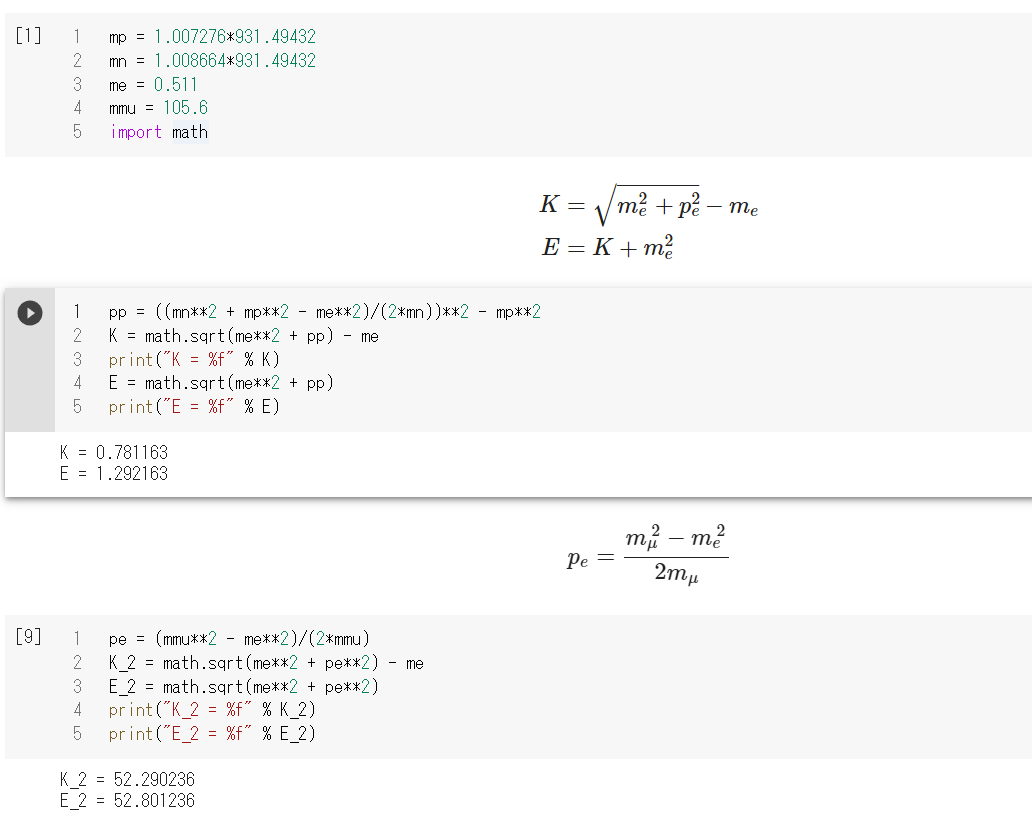
\includegraphics[width=0.9\linewidth]{maxT.png}
	\caption{Pythonでの実行結果}
	\label{fig:max_T}
\end{figure}

\subsubsection*{別解}
四元運動量の保存を用いる。問題設定より、$p_n = (m_n,\,0),\,p_p=(E_p,\,\va{p}_p),\,p_e=(E_e,\,\va{p}_e),\,p_{\nu}=(E_{\nu},\,E_{\nu})$となる。
$p_n = p_p + p_e + p_\nu$となる。$\va{p}_e$が最大になるのは、$\va{p}_p = -\va{p}_e$になり、$E_{\nu}=0$であるときなので、2通りのやりかたで四元ベクトルの2乗を計算すると、
\begin{align}
	0     & = (p_n-p_p-p_e)^2 = (m_n - E_p - E_e)^2 \Longrightarrow E_e = m_n-E_p                                 \\
	p^2_e & = (p_n-p_p)^2 = m_e^2 = m_n^2 + m_p^2 - 2m_nE_p  \Longrightarrow E_p = \frac{m_n^2+m_p^2-m_e^2}{2m_n}
\end{align}
を得る。したがって、
\begin{equation}
	E_e = m_n - E_p = \frac{m_n^2-m_p^2+m_e^2}{2m_n},\,K_e = E_e-m_e = \frac{(m_n-m_e)^2 - m_p^2}{2m_n}
\end{equation}
となる。
\subsubsection*{補足}
$\mu$粒子崩壊時に生成される電子のエネルギー分布の理論式は、\cite{6}の第2章によると、以下のようにして求められる:

$\mu$粒子の崩壊振幅を$M$とすると、
\begin{equation}
	M =\frac{g_w^2}{8(M_wc)^2}\qty[u(3)\gamma^\mu(1-\gamma^5)u(1)]\qty[u(4)\gamma_\mu(1-\gamma^5)u(2)]
\end{equation}
と与えられる。
$g_w$は弱い相互作用の結合定数、$M_w$はウィークボソンの質量、$\gamma^5=i\gamma^0\gamma^1\gamma^2\gamma^3$はガンマファイブであり、
$u(i);\,1\leq i\leq 4$はディラック方程式の解となるスピノールである。
これより、四元運動量を用いて
\begin{equation}
	\ev{M^2} = 2\qty(\frac{g_w}{M_wc})^4(p_\mu p_e)(p_{\nu_\mu}p_{\nu_e})
\end{equation}
と計算できる。崩壊幅を$\dd{\Gamma}$とすると、
\begin{equation}
	\dv{\Gamma}{E} = \frac{\ev{M^2}c}{(4\pi)^4hm_{\mu}}\dd{E}_e\frac{\dd[3]{\va{p}_{\nu_{e}}}}{E_{\nu_{e}}^2}
\end{equation}
となり、最終的に
\begin{equation}
	\dv{\Gamma}{E} = \qty(\frac{g_w}{M_wc})^4\frac{m_\mu^2 E^2}{2h(4\pi)^3}\qty(1-\frac{4E}{3m_{\mu}c^3})
\end{equation}
を得る。(計算は丁寧に記載されていたが、途中から$E_{\nu_e}\to E_{e}$と変化しており、よくわからなかった。)これが$\mu$粒子崩壊時の電子のエネルギー分布を表す。
なお、崩壊幅とは崩壊率のことであり、平均寿命$\tau$に対して$\Gamma = \hbar/\tau$と定義される。

\newpage
\begin{tcolorbox}[
		colback = white,
		colframe = green!35!black,
		fonttitle = \bfseries]
	\begin{mondai}[1-5]
		\ce{^{184}W}の密度分布は式\eqref{eq:woods}で与えられる。$c,\,z$の値は表4-1を参照し($c=6.51,\,z=0.545$)、原子核の平均密度を求めよ。
	\end{mondai}
\end{tcolorbox}

\begin{kaitou}
	(以下は自分の試行錯誤を残しているだけである。本来の解答は次ページから始まっている。)
	核物質密度$\rho_0=\SI{0.16}{nucleons/fm^3}$を用いると、
	\begin{equation}
		\rho(r) = \frac{\rho_0}{1+\exp\qty({(r-c)}/{z})}
	\end{equation}
	である。平均密度を$\bar{\rho}$とすると、
	\begin{equation}
		4\pi\int_0^{\infty}dr\,\frac{\rho_0r^2}{1+\exp\qty({(r-c)}/{z})} = \frac{4}{3}\pi (r_0A^{1/3})^3\bar{\rho}
	\end{equation}
	が成立する。ここで、
	\begin{equation}
		I = \int_0^{c}dr\,\frac{r^2}{1+\exp((r-c)/z)} + \int_c^{\infty}dr\,\frac{r^2}{1+\exp((r-c)/z)}
	\end{equation}
	と置く。第一項については、$c/z\gg 1$より
	\begin{equation}
		45.91= \frac{c^3}{6} =\frac{1}{2}\int_0^cdr\,r^2 \leq \int_0^{c}dr\,\frac{r^2}{1+\exp((r-c)/z)} \leq \int_0^cdr\,r^2 = \frac{c^3}{3} = 92.0
	\end{equation}
	が成立する。第二項を計算するために、以下の積分を考える:
	\begin{equation}
		J(k) = \int_0^\infty dx\, \frac{x^k}{1+e^x} = \int_0^\infty x^ke^{-x}\qty(1-e^{-x}+e^{-2x}+e^{-3x}+\cdots)
		= -\sum_{n=1}^\infty(-1)^n\int_0^\infty dx\,x^ke^{-nx}\;。
	\end{equation}
	ここで、$x\geq 0$で成立する等式$(1+e^{-x})^{-1} = 1-e^{-x}+e^{-2x}+e^{-3x}+\cdots$を用いた。
	\begin{equation}
		\int_0^\infty dx\,x^ke^{-nx} = \frac{\Gamma(k+1)}{n^{k+1}}
	\end{equation}
	が成立するため、
	\begin{equation}
		J(k) = -k!\sum_{n=1}^{\infty}\frac{(-1)^n}{n^{k+1}} \eqqcolon -k!A(k)
	\end{equation}
	とおける。ゼータ関数$\zeta(k)=\sum_{n=1}^{\infty}n^{-k}$を用いると
	\begin{equation}
		\zeta(k+1)+A(k) = \sum_{n=1}^{\infty}\frac{2}{(2n)^{k+1}} = \frac{\zeta(k+1)}{2^k}\Longrightarrow J(k) = -k!A(k) = k!\qty(1-\frac{1}{2^k})\zeta(k+1)\quad(k\geq 1)
	\end{equation}
	が成立する。また、$J(0) = \ln{2}$(メルカトル級数)になる。以上より、
	\begin{equation}
		J(0) = \ln{2}=0.69,\,J(1) = \frac{1}{2}\zeta(2)=\frac{1.64}{2},\,J(2) = \frac{3}{2}\zeta(3) = \frac{3*1.20}{2}
	\end{equation}
	を得る。これで$I$の第二項を求める準備が整った。$(r-c)/z = u$とおくと、$dr = zdu,\,r = zu+c$となるため、
	\begin{equation}
		\int_c^{\infty}dr\,\frac{r^2}{1+\exp((r-c)/z)} = \int_0^{\infty}(zdu)\,\frac{z^2u^2+2zcu+c^2}{1+e^u} = z^3J(2)+2z^2cJ(1)+zc^2J(0) = \SI{18.97}{fm^3}
	\end{equation}
	となる。したがって、$65\leq I \leq 111$と評価できる。

	\subsection*{ゾンマーフェルト展開で計算する方法}
	第一項の値が求まらないなぁと友達に言ったら、そもそもゾンマーフェルト展開できるんじゃない?と言われたので、以下ではゾンマーフェルト展開を用いて(同じ道筋をたどって)積分値を求める。
	ゾンマーフェルト展開とは、フェルミ分布関数がデルタ関数的な変化をすることに着目し、部分積分を行う低温展開方法であったので、
	\begin{align}
		I & = z\int_{-c/z}^{\infty}dx\,\frac{(zx+c)^2}{1+e^x} = \qty[\frac{(zx+c)^3}{3}\frac{1}{1+e^x}]_{-c/z}^{\infty} + \int_{-c/z}^{\infty}dx\,\frac{(zx+c)^3}{3}\frac{e^x}{(1+e^x)^2} \\
		  & \approx \int_{-\infty}^{\infty}\,dx\frac{c^3+3cz^2x^2}{3}\underset{\text{偶関数}}{\frac{e^x}{(1+e^x)^2}} = \frac{c^3}{3} + 2cz^2\int_0^{\infty}dx\,\frac{x^2e^x}{(1+e^x)^2}
	\end{align}
	を得る。補正項は
	\begin{equation}
		\int_{0}^{\infty}dx\,\frac{x^2e^x}{(1+e^x)^2} = \qty[2x\frac{-1}{1+e^x}]_{0}^{\infty}+\int_0^\infty dx\,\frac{2x}{1+e^x} = \frac{\pi^2}{6}
	\end{equation}
	となるため、最終的に
	\begin{equation}
		I =\frac{c^3}{3} + \frac{cz^2\pi^2}{3} = 98.2
	\end{equation}
	を得る。Wolfram alphaを用いて厳密に積分した結果、$I=98.3262$となり、良い精度で一致していた。

	\subsubsection*{自分のメモ用}
	$I$の値のうち、$c^3/3$の項は$0\leq r\leq c$でフェルミ分布関数が$1$とみなしたときの値である。よって、$I$のうち、$c\leq r$で積分した値(有限温度の効果にあたるもの)は$cz^2\pi^2/3=6.23$となる(と思った)。
	これは、上で厳密に得た値$18.97$と異なる。そのため、ゾンマーフェルト展開は妥当ではないのではと思ったが、この議論は間違っている。
	下図を見ればわかるように、ゾンマーフェルト展開の補正項は、(フェルミ分布関数の補正)$\times$(係数関数)の積分を表しているため、単純に$c\leq r\leq \infty$で積分した値とは異なる。
	\begin{figure}[H]
		\centering
		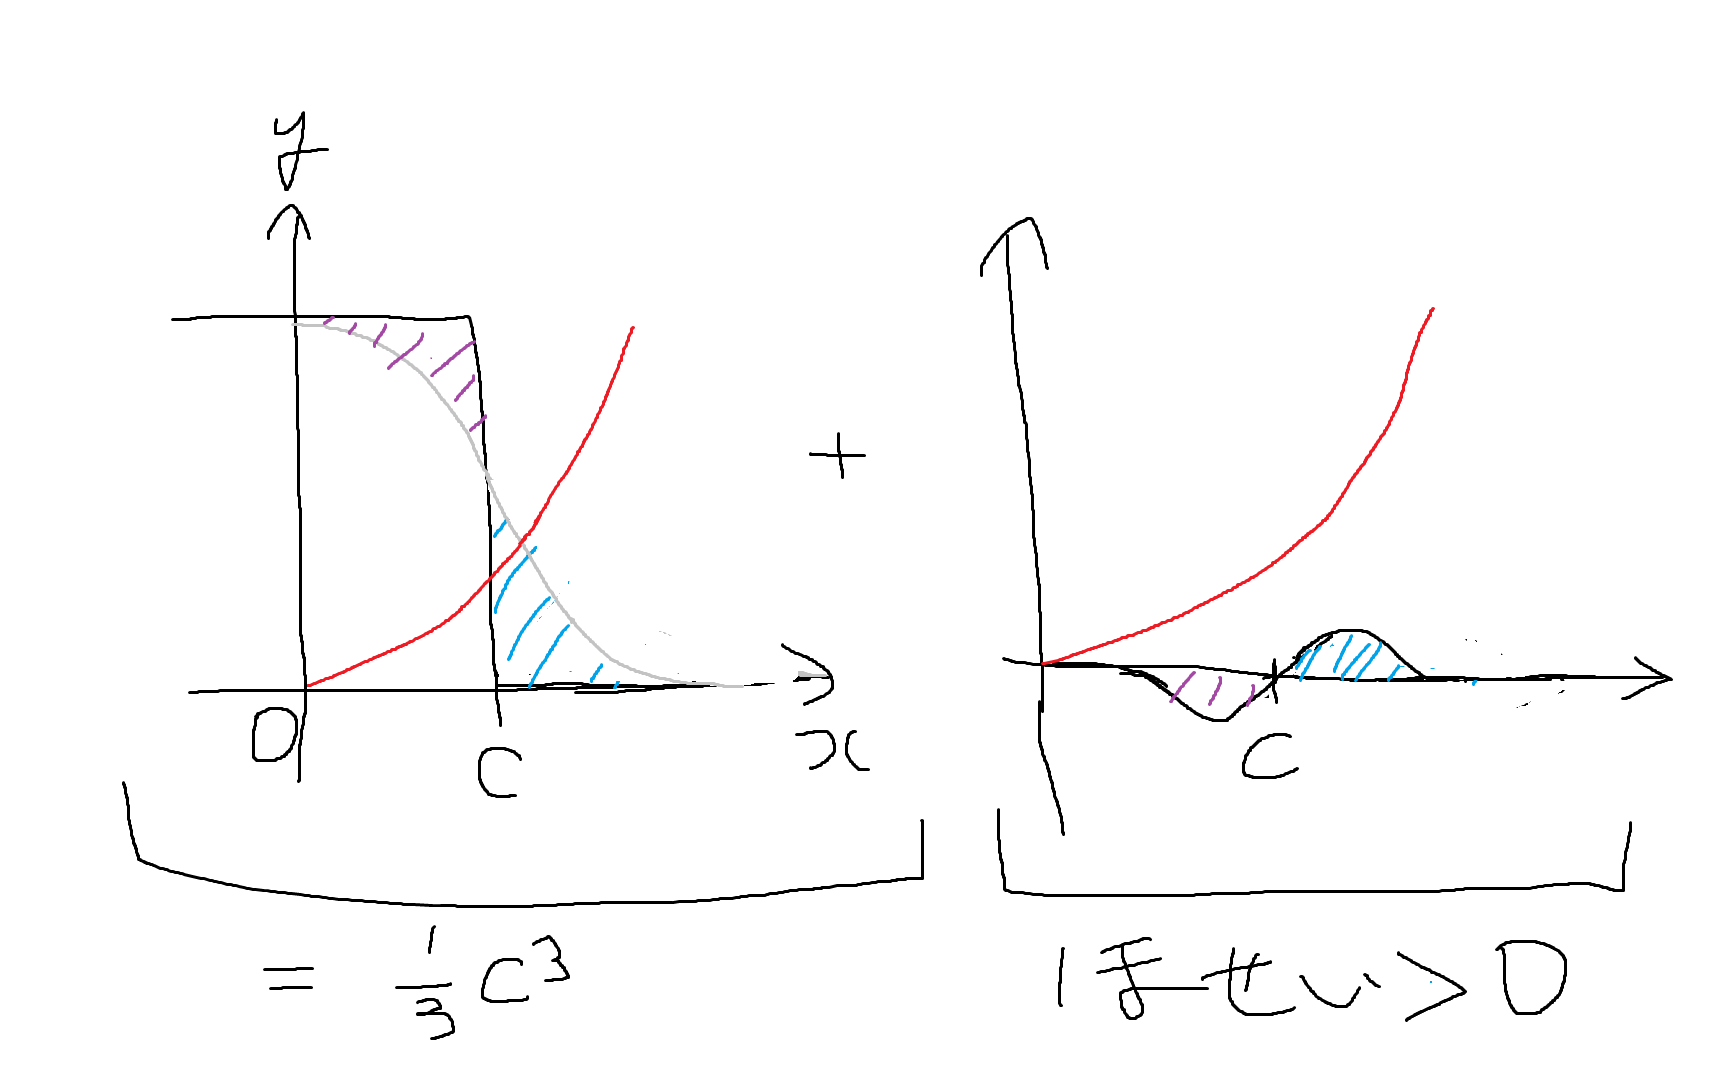
\includegraphics[width=0.7\linewidth]{zonmar.png}
		\caption{ゾンマーフェルト展開がしていること}
		\label{fig:zonmar}
	\end{figure}

	以上の計算によって、
	\begin{equation}
		\bar{\rho} = \frac{3I}{r_0^3A}\rho_0= \frac{3*\SI{98.2}{fm^3}}{(1.2)^3\,\si{fm^3}*184}\times\SI{0.16}{nucleons/fm^3} = \SI{0.14}{nucleons/fm^3}
	\end{equation}
	を得る。これは、式\eqref{eq:0.14}と同じ値である。
\end{kaitou}

\vskip\baselineskip
\begin{tcolorbox}[
		colback = white,
		colframe = green!35!black,
		fonttitle = \bfseries]
	\begin{mondai}[1-6]
		\ce{^{56}Fe}では、準位密度パラメータは$a=\SI{7.2}{MeV^{-1}}$と知られている。励起エネルギーが$E=\SI{20}{MeV}$の場合の準位密度を求めよ。
	\end{mondai}
\end{tcolorbox}

\begin{kaitou}
	\begin{equation}
		\rho_{\text{A}}(E) = \frac{1}{12a^{1/4}E^{5/4}}e^{2\sqrt{aE}} = 195.7\quad\text{@}\SI{20}{MeV}
	\end{equation}
\end{kaitou}


\section{補足:励起状態の状態密度の計算について}
\cite{3}のpp.84-pp.85にかけて、励起状態の準位密度の計算が紹介されていた。(より具体的にはA.Bohr and B.R.Mottelson: Nuclear Structure, Vol 1(日本語訳版は『原子核構造$\langle1\rangle$ 単一粒子運動』)に掲載されている。)
以下の計算は自分で追ったのではなく、教科書の丸写しである。

A核子系の励起エネルギー$E$での準位密度は、固有エネルギー$E_n(A)$を用いて
\begin{equation}
	\hat\rho(E,\,A) = \sum_{A'}\sum_n\delta(A-A')\delta(E-E_n(A))
\end{equation}
で定義される。(なぜ$A'$についての和を取るのか?)
この$\hat{\rho}(E,\,A)$は大分配関数$Z(\alpha,\,\beta)$と
\begin{equation}
	Z(\alpha,\,\beta) = \int\dd{E}\int\dd{A}\hat{\rho}(E,\,A)e^{\alpha A-\beta B}
\end{equation}
の関係にあるため、$Z(\alpha,\,\beta)$がわかれば逆Laplace変換によって$\hat{\rho}(E,\,A)$を得られる:
\begin{equation}
	\hat{\rho}(E,\,A) = \frac{1}{(2\pi i)^2}\iint_{-i\infty}^{i\infty}Z(\alpha,\,\beta)e^{\beta E - \alpha A}\dd{\alpha}\dd{\beta}\;。
\end{equation}
被積分関数の指数$S(\alpha,\,\beta) = \beta E - \alpha A + \ln{Z(\alpha,\,\beta)}$はエントロピーに対応し、積分変数$\alpha,\,\beta$に関して急激に変化する関数である。
そこで、$S(\alpha,\,\beta)$の平衡点まわりで展開して2次まで考慮する鞍点法を採用すると、$E$に関して離散的な準位密度$\hat{\rho}(E,\,A)$から、$E$とともに滑らかに変化する準位密度${\rho}(E,\,A)$が得られる。
つまり、
\begin{equation}
	\hat{\rho}(E,\,A)\longrightarrow \rho(E,\,A) = \frac{1}{2\pi\sqrt{D(\alpha,\,\beta)}}e^{S(\alpha,\,\beta)}
\end{equation}
となる。ただし、$(\alpha,\,\beta)$を平衡点としており、
\begin{equation}
	D(\alpha,\,\beta) =
	\begin{vmatrix}
		\pdv[2]{\ln{Z}}{\beta}         & \pdv[2]{\ln{Z}}{\alpha}{\beta} \\
		\pdv[2]{\ln{Z}}{\beta}{\alpha} & \pdv[2]{\ln{Z}}{\alpha}
	\end{vmatrix}
\end{equation}
である。以上の一般論をFermi気体模型に適用し、角運動量$I$、パリティ$\pi$をもつ準位の密度を計算すると、$N=Z=A/2$の場合、
\begin{equation}
	\rho(A,\,E,\,I,\,\pi) =  \frac{2I+1}{24}a_{\text{F}}^{1/2}\qty(\frac{\hbar^2}{2\mathscr{I}_{\text{rig}}})^{3/2}\qty(E-\frac{\hbar^2}{2\mathscr{I}_{\text{rig}}} I(I+1))^{-2}
	\exp\qty{2\sqrt{a_{\text{F}}\qty(E-\frac{\hbar^2}{2\mathscr{I}_{\text{rig}}}I(I+1))}}
\end{equation}
を得る\footnote{$\mathscr{I}_{\text{rig}}$は原子核と同じ密度分布を持つ剛体の慣性モーメント}。パラメータ$a_{\text{F}}$は
\begin{equation}
	a_{\text{F}} = \frac{\pi^2}{6}g(e_{\text{F}}) = \frac{\pi^2}{4}\frac{A}{e_{\text{F}}} = \frac{A}{15}\,\si{MeV^{-1}}
\end{equation}
と与えられる。なお、1粒子準位の密度$g(e) = \sum_i\delta(e-e_i)$がFermiエネルギー$e_{\text{F}}$近傍で一定と近似した。
この$a_{\text{F}}$は実験値$a\approx A/8$の約半分である。このことから、殻構造や集団励起など、核表面に関わる効果の重要性が現れている。







\begin{thebibliography}{9}
	\bibitem{3} 市村宗武・坂田文彦・松柳研一, 『岩波講座 現代の物理学9 原子核の理論』, 岩波書店.
	\bibitem{6} 池田侑加・坂本朋子, 卒業論文『ミュー粒子の寿命と崩壊電子エネルギースペクトラムの研究』. \url{https://webhepl.cc.nara-wu.ac.jp/old_HP/thesis/4kaisei/2015/2015_ikeda_sakamoto_sotsugyouronbun.pdf}
	\bibitem{1} 原子核の基礎的なことを参考にしたサイト1 \url{http://ne.phys.kyushu-u.ac.jp/ne.phys.kyushu-u.ac.jp/wakasa/public_html/np17/np6.pdf}
	\bibitem{2} 原子核の基礎的なことを参考にしたサイト2 \url{https://www.mns.kyutech.ac.jp/~okamoto/education/nuclearpower/nucleus-properties-text091104.pdf}
	\bibitem{4} ベータ崩壊の計算法の参考その1 \url{https://hepweb.ucsd.edu/ph110b/110b_notes/node63.html}
	\bibitem{5} ベータ崩壊の計算法の参考その2 \url{http://websites.umich.edu/~ners311/CourseLibrary/bookchapter15.pdf}
\end{thebibliography}

\end{document}